29. \begin{figure}[ht!]
\center{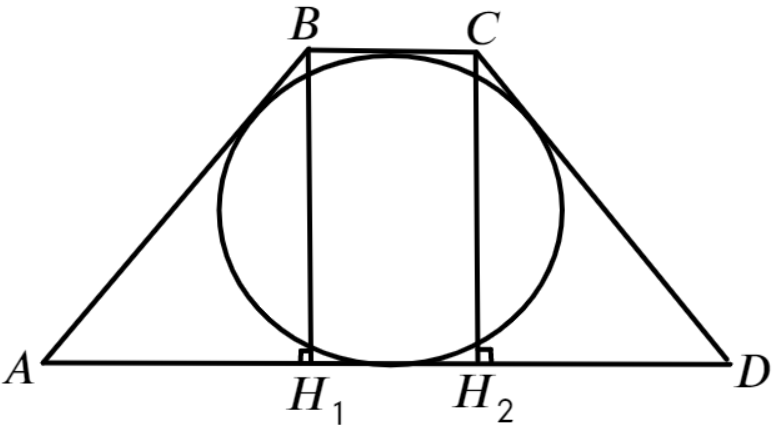
\includegraphics[scale=0.35]{g8-29.png}}
\end{figure}\\
Так как трапеция является описанным четырёхугольником, суммы его противоположных сторон равны. Так как она равнобедренная, $2AB=2CD=BC+AD=36+100=136,\ AB=CD=68$см. Опустим две высоты $BH_1$ и $CH_2,$ тогда $H_1H_2=BC=36$см, $AH_1=DH_2=(100-36):2=32$см. По теореме Пифагора $BH_1=\sqrt{68^2-32^2}=60$см. Тогда $R=BH_1:2=60:2=30$см.\\
